\chapter{Data exploration}


\section{The datasets}
Rakuten France provided a dataset consisting of approximately 99 000 product listings in CSV format. This dataset includes both the training set with 84 916 entries and the test set with 13 812 entries. Each entry comprises product designations, product descriptions, product images, and their corresponding product type code.

The datasets are organized based on two criteria: training or test and input or output. The data is available in three distinct csv files:

\begin{enumerate}
    \item X train.csv: Training input file
    \item Y train.csv: Training output file
    \item X test.csv: Test input file
\end{enumerate}

The images.zip file contains all the images. Extracting this file results in a folder named "images" with two subfolders, "image training" and "image test," containing training and test images, respectively.

\subsection{X train.csv}
The input files follow the common CSV format, where the first line serves as the header, and columns are delimited by commas. The columns in these files include an integer ID for product identification, a product designation providing a concise product summary, a more detailed product description (which may contain NaN values for products lacking this information), a unique product ID (productid), and a unique image ID (imageid).

\subsection{Y train.csv}
Turning attention to Y train, it contains two columns : an integer ID for product identification and the product type code.

\subsection{Y test.csv}
The X test table mirrors the structure of X train, serving as a dataset for Rakuten to assess the performance of the chosen model. With 84,916 observations or products and four variables, X test reflects the same information as X train

\section{Data visualization}
In an effort to comprehend the dataset's composition before visualization, it was imperative to explore its structure and understand the distribution of key attributes.\\

\subsection{Columns composition}
First of all, there are several empty values in the description column, which means that not all products are uploaded with a description. \\


\begin{figure}[h]
    \centering
    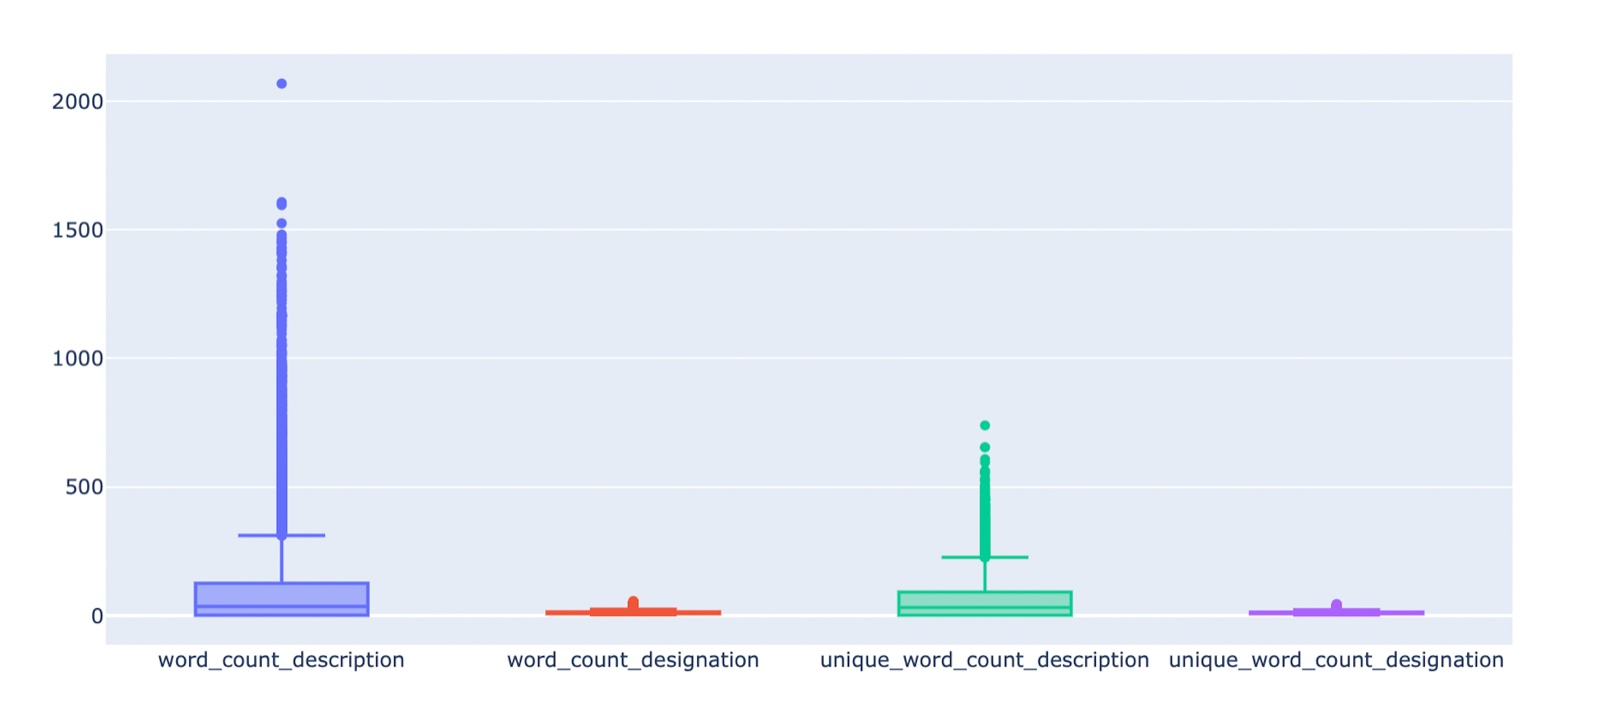
\includegraphics[width=1\textwidth]{word_count.jpeg}
    \caption{Word Counts for Both Designation and Description.}
    \label{fig:word_count}
\end{figure}

The graph shows that despite the significant difference between the word count for description and that of designation, that same difference isn't as important for the unique word count. \\
This comparison between the "description" and "designation" variables indicates that the "description" column likely contains a significant amount of information, despite the presence of a substantial number of NaNs (missing values). Therefore, we should refrain from removing this column during the handling of missing values. We will take that into consideration while coding our model. Some inputs will have more furnished features than others. \\

\subsection{Product categories}
Moreover, it is revealed that all products in X train have been categorized into 27 different product types, each identified by a unique numeric code. The dataset exhibits a light imbalance due to varying observation counts across these categories.
The following graphics demonstrate that : \\

\newpage

\begin{figure}[h]
    \centering
    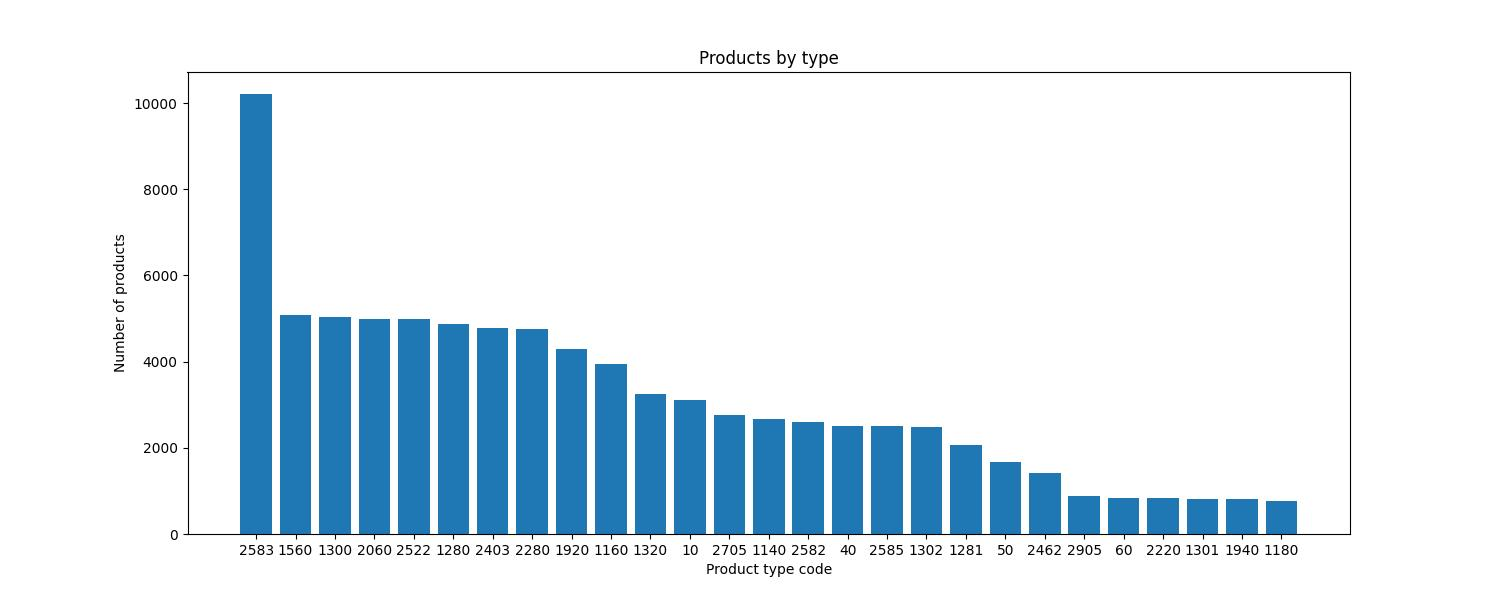
\includegraphics[width=1\textwidth]{bar_plot.jpeg}
    \caption{Number of products per category.}
    \label{fig:nproduct}
\end{figure}


To see how different product types are distributed, we can use a pie chart. \\

\begin{figure}[h]
    \centering
    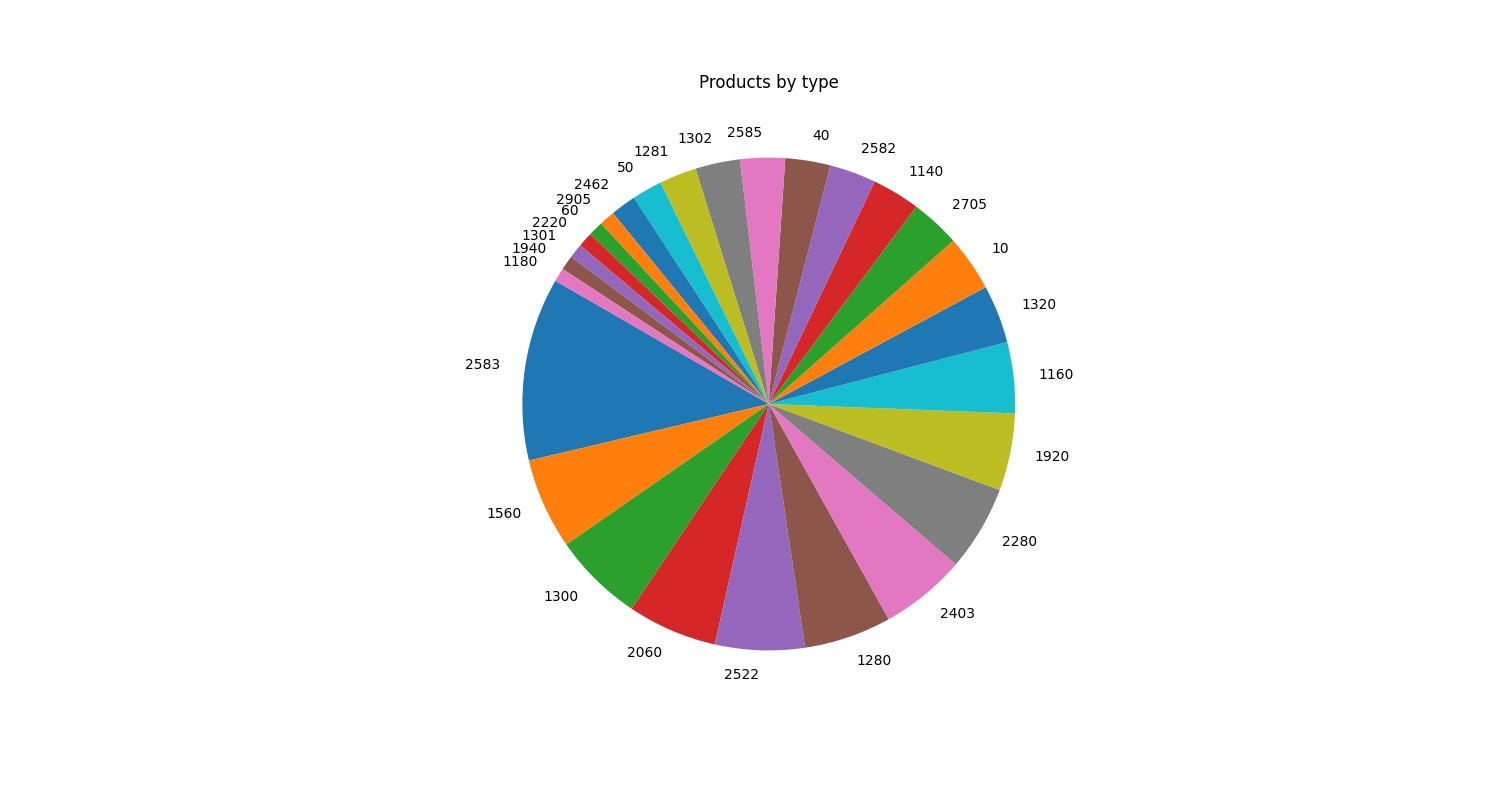
\includegraphics[width=1\textwidth]{pie_plot.jpeg}
    \caption{Distribution of products per category}
    \label{fig:product}
\end{figure}


We can see that category '2583' contributes significantly to the whole compared to other categories.On the other hand, the categories with the smallest number of samples will be more challenging to detect. We have an unbalanced dataset as the number of observations is not the same for all categories. This should be taken into account during modeling.

\newpage
\subsection{U-map}

As the UMAP algorithm takes numerical input, certain modifications were applied to the "designation" column to facilitate its integration into the analysis:  the code we have on the notebook systematically cleans the text by removing digits, punctuation, diacritics, HTML tags, and URLs. The text is then converted to lowercase, tokenized using NLTK's word tokenizer, and further processed with Keras Tokenizer, which filters out specified characters. Additionally, the sequences of tokenized words are padded using Keras' pad sequences function to ensure uniform length. Two new columns, 'designation sequences' and 'designation padded', are created in the DataFrame to store the intermediate and final processed text, making it suitable for subsequent analysis or machine learning tasks. \\

A UMAP plot was generated to explore the underlying structure of the dataset. The plot revealed distinct clusters, some of which were readily identifiable, while others appeared less defined. Outliers were also observed, indicating certain products or groups of products that deviate significantly from the main clusters.

